\section{Overview on Development Setup}

A setup for development is explained in table~\ref{tab:requirements}. The most basic components are 
required for hands-on development. Main issue is a python interpreter and common libraries.\footnote{For example
CherryPy, pyserial and optionally a module for SQL-bindings in Python.}

Figure~\ref{setupic} shows the last version of the used development system. The keyboard and monitor on the host machine
is just used to monitor debug output and use the included \textsl{interactive} mode on the \textsc{WSN}.\footnote{So you can 
type in commands meant for nodes on the host machine instead of using the RESTful http-access}

\ref{nodepic} and \ref{hostpic} show the expected results after a clean startup. The controller identifies itself with a
self-chosen name and exchanges basic data for database population.
 

\begin{table}[h] 
\centering 
\begin{tabular}{|l||l|} 
General Component & Specific Component\\ 
\hline 
i86 host machine & 300MHz, 512MB\\ 
host OS & Debian stable(Squeeze) \\ 
Python Interpreter & Python 2.7 with pyserial \\ 
Database & MySQL\footnote{A local SQLite version with reduced functionality has no additional requirements} \\ 
1 Wireless Sensor Node as Controller & Renesas ZMD28-BRD \\
n Wireless Sensor Node as Client & Renesas ZMD28-BRD \\ 
\end{tabular} 
\caption{ Table of Requirements} 
\label{tab:requirements} 
\end{table}


\begin{figure}[H]
   \centering
   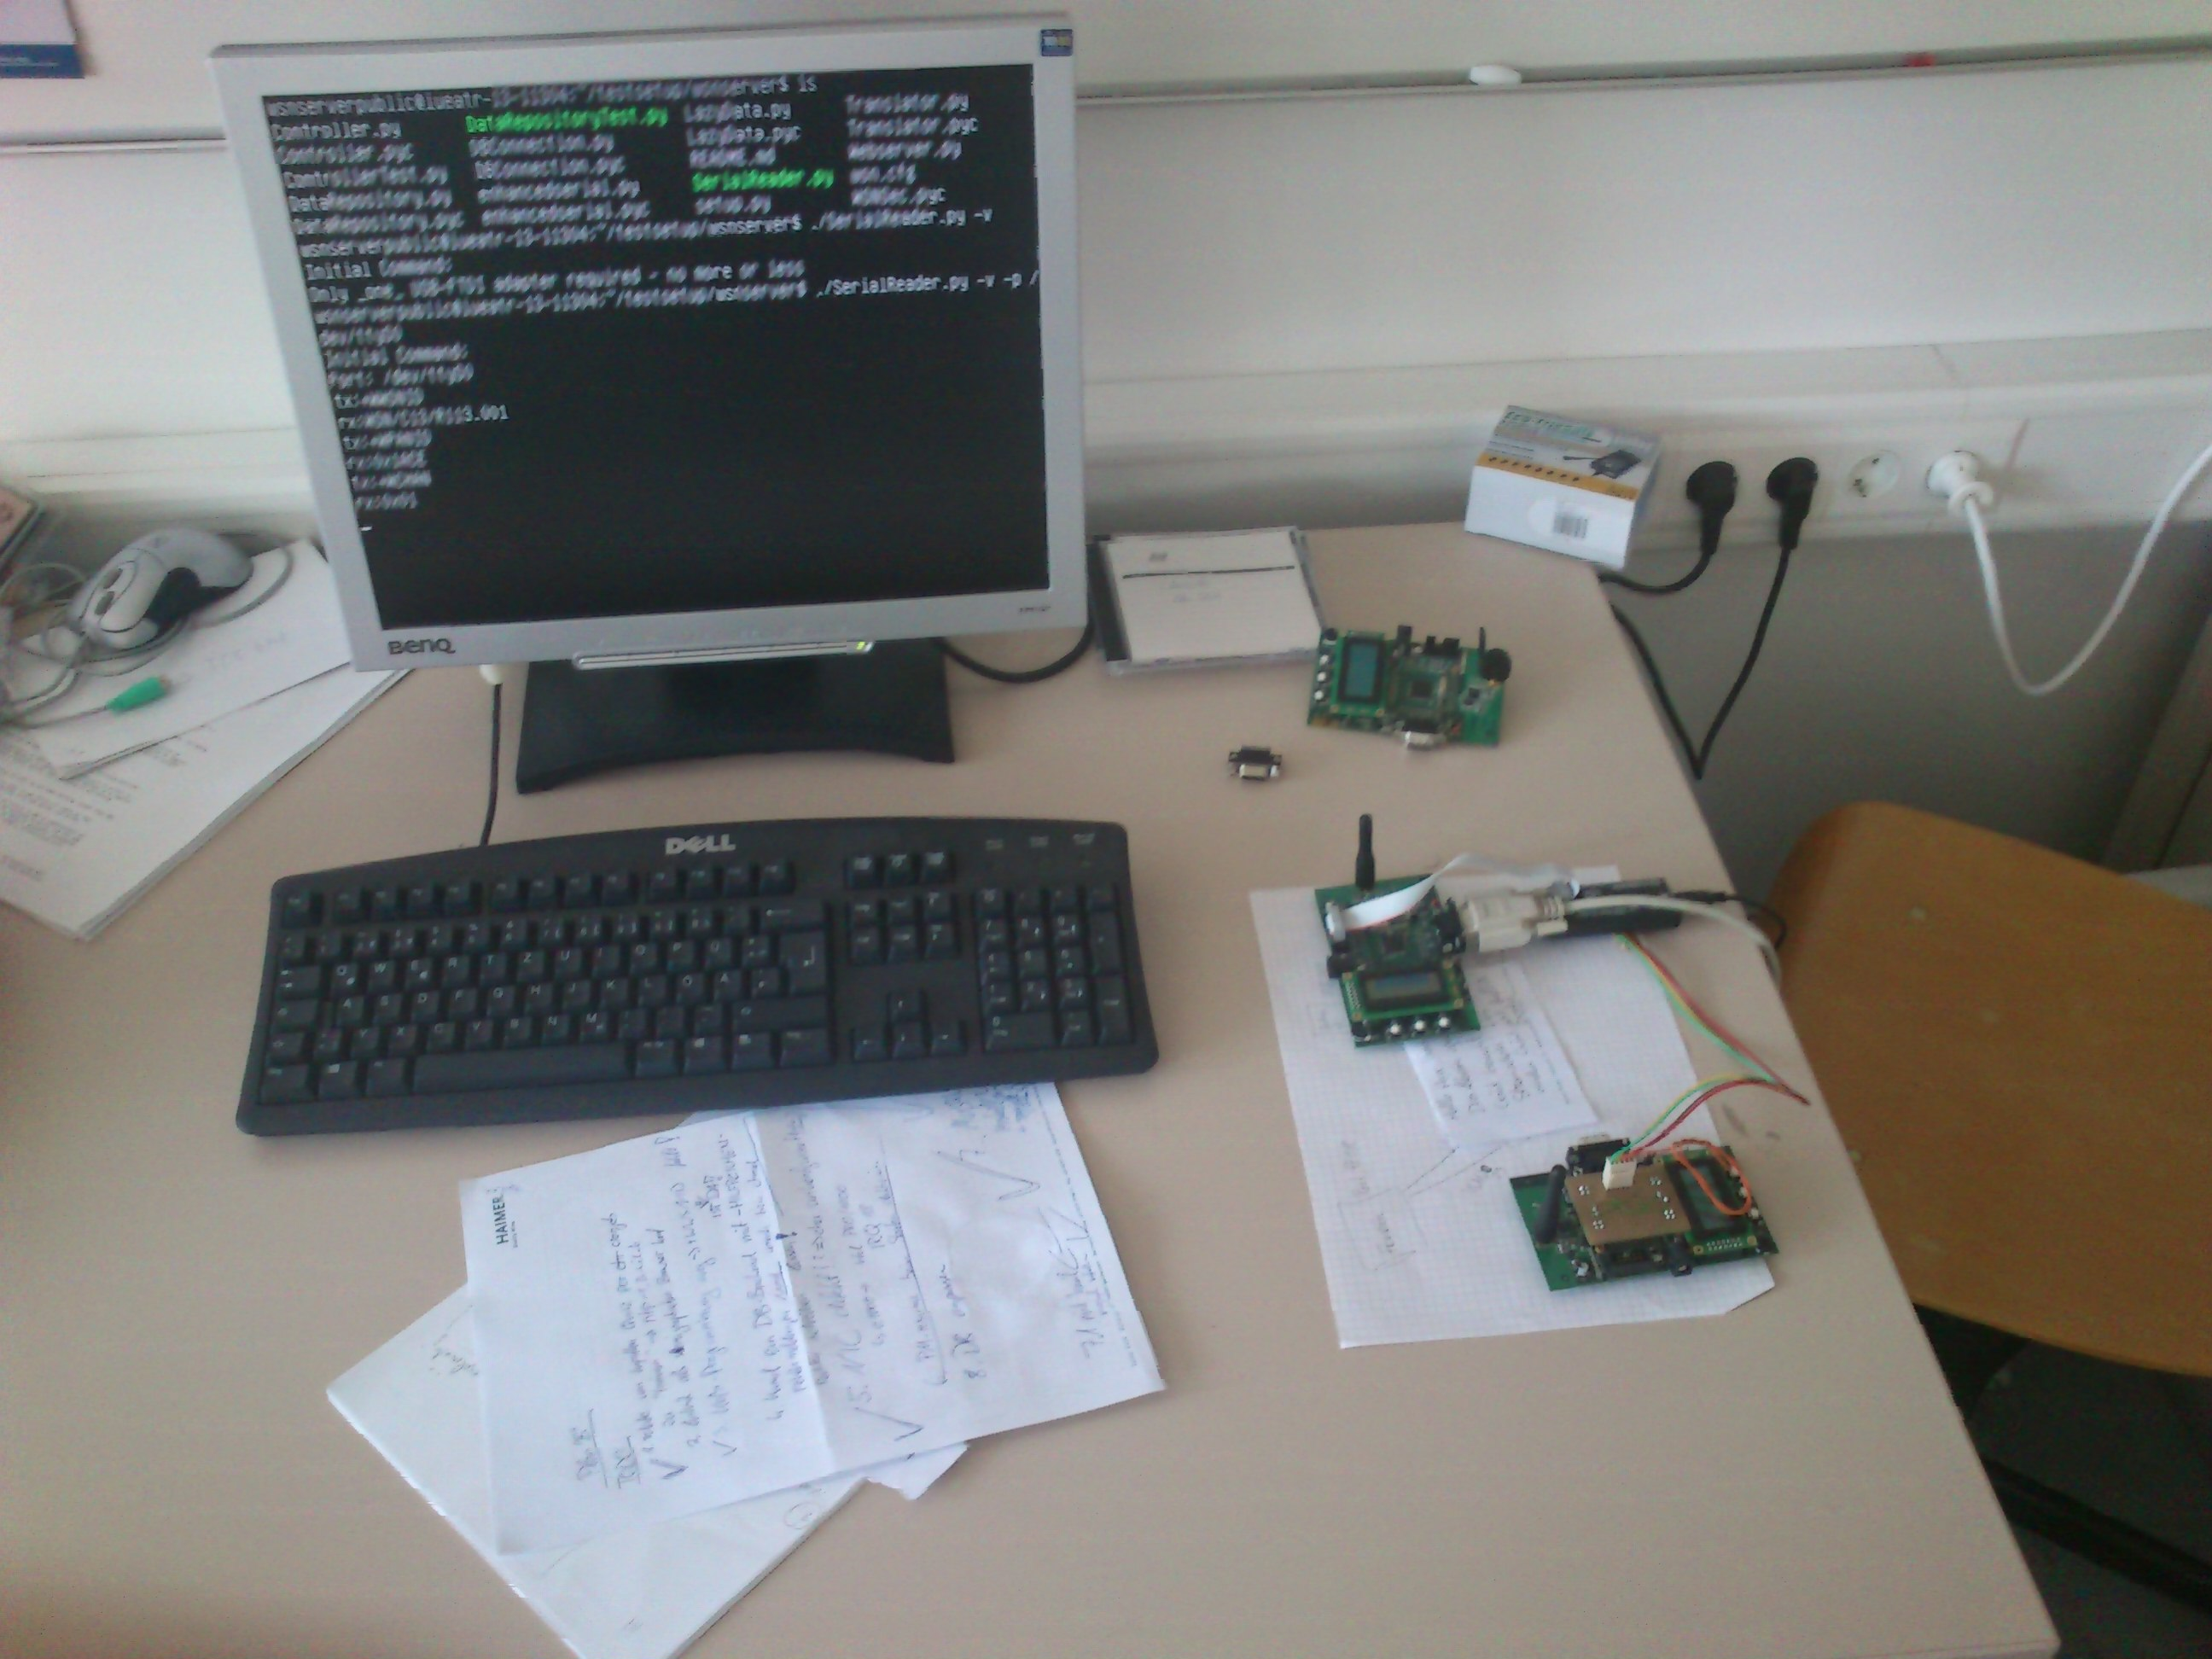
\includegraphics[width=0.8\textwidth]{pic/whole_setup.jpg}%
   \caption{Glimpse on the development setup}
   \label{setupic}%
\end{figure}

A disc image will be distributed along this document but a download is also available.\footnote{\url{XXXXXXXXXXXXXX} and use 
\url{http://clonezilla.org} as your tool of restoration.}

Look up on chapter~\ref{sec:install} on page~\pageref{sec:install} for detailed installation instructions without using the disc image.

For general x86-machine there are not specific demands 

\begin{figure}[H]
   \centering
   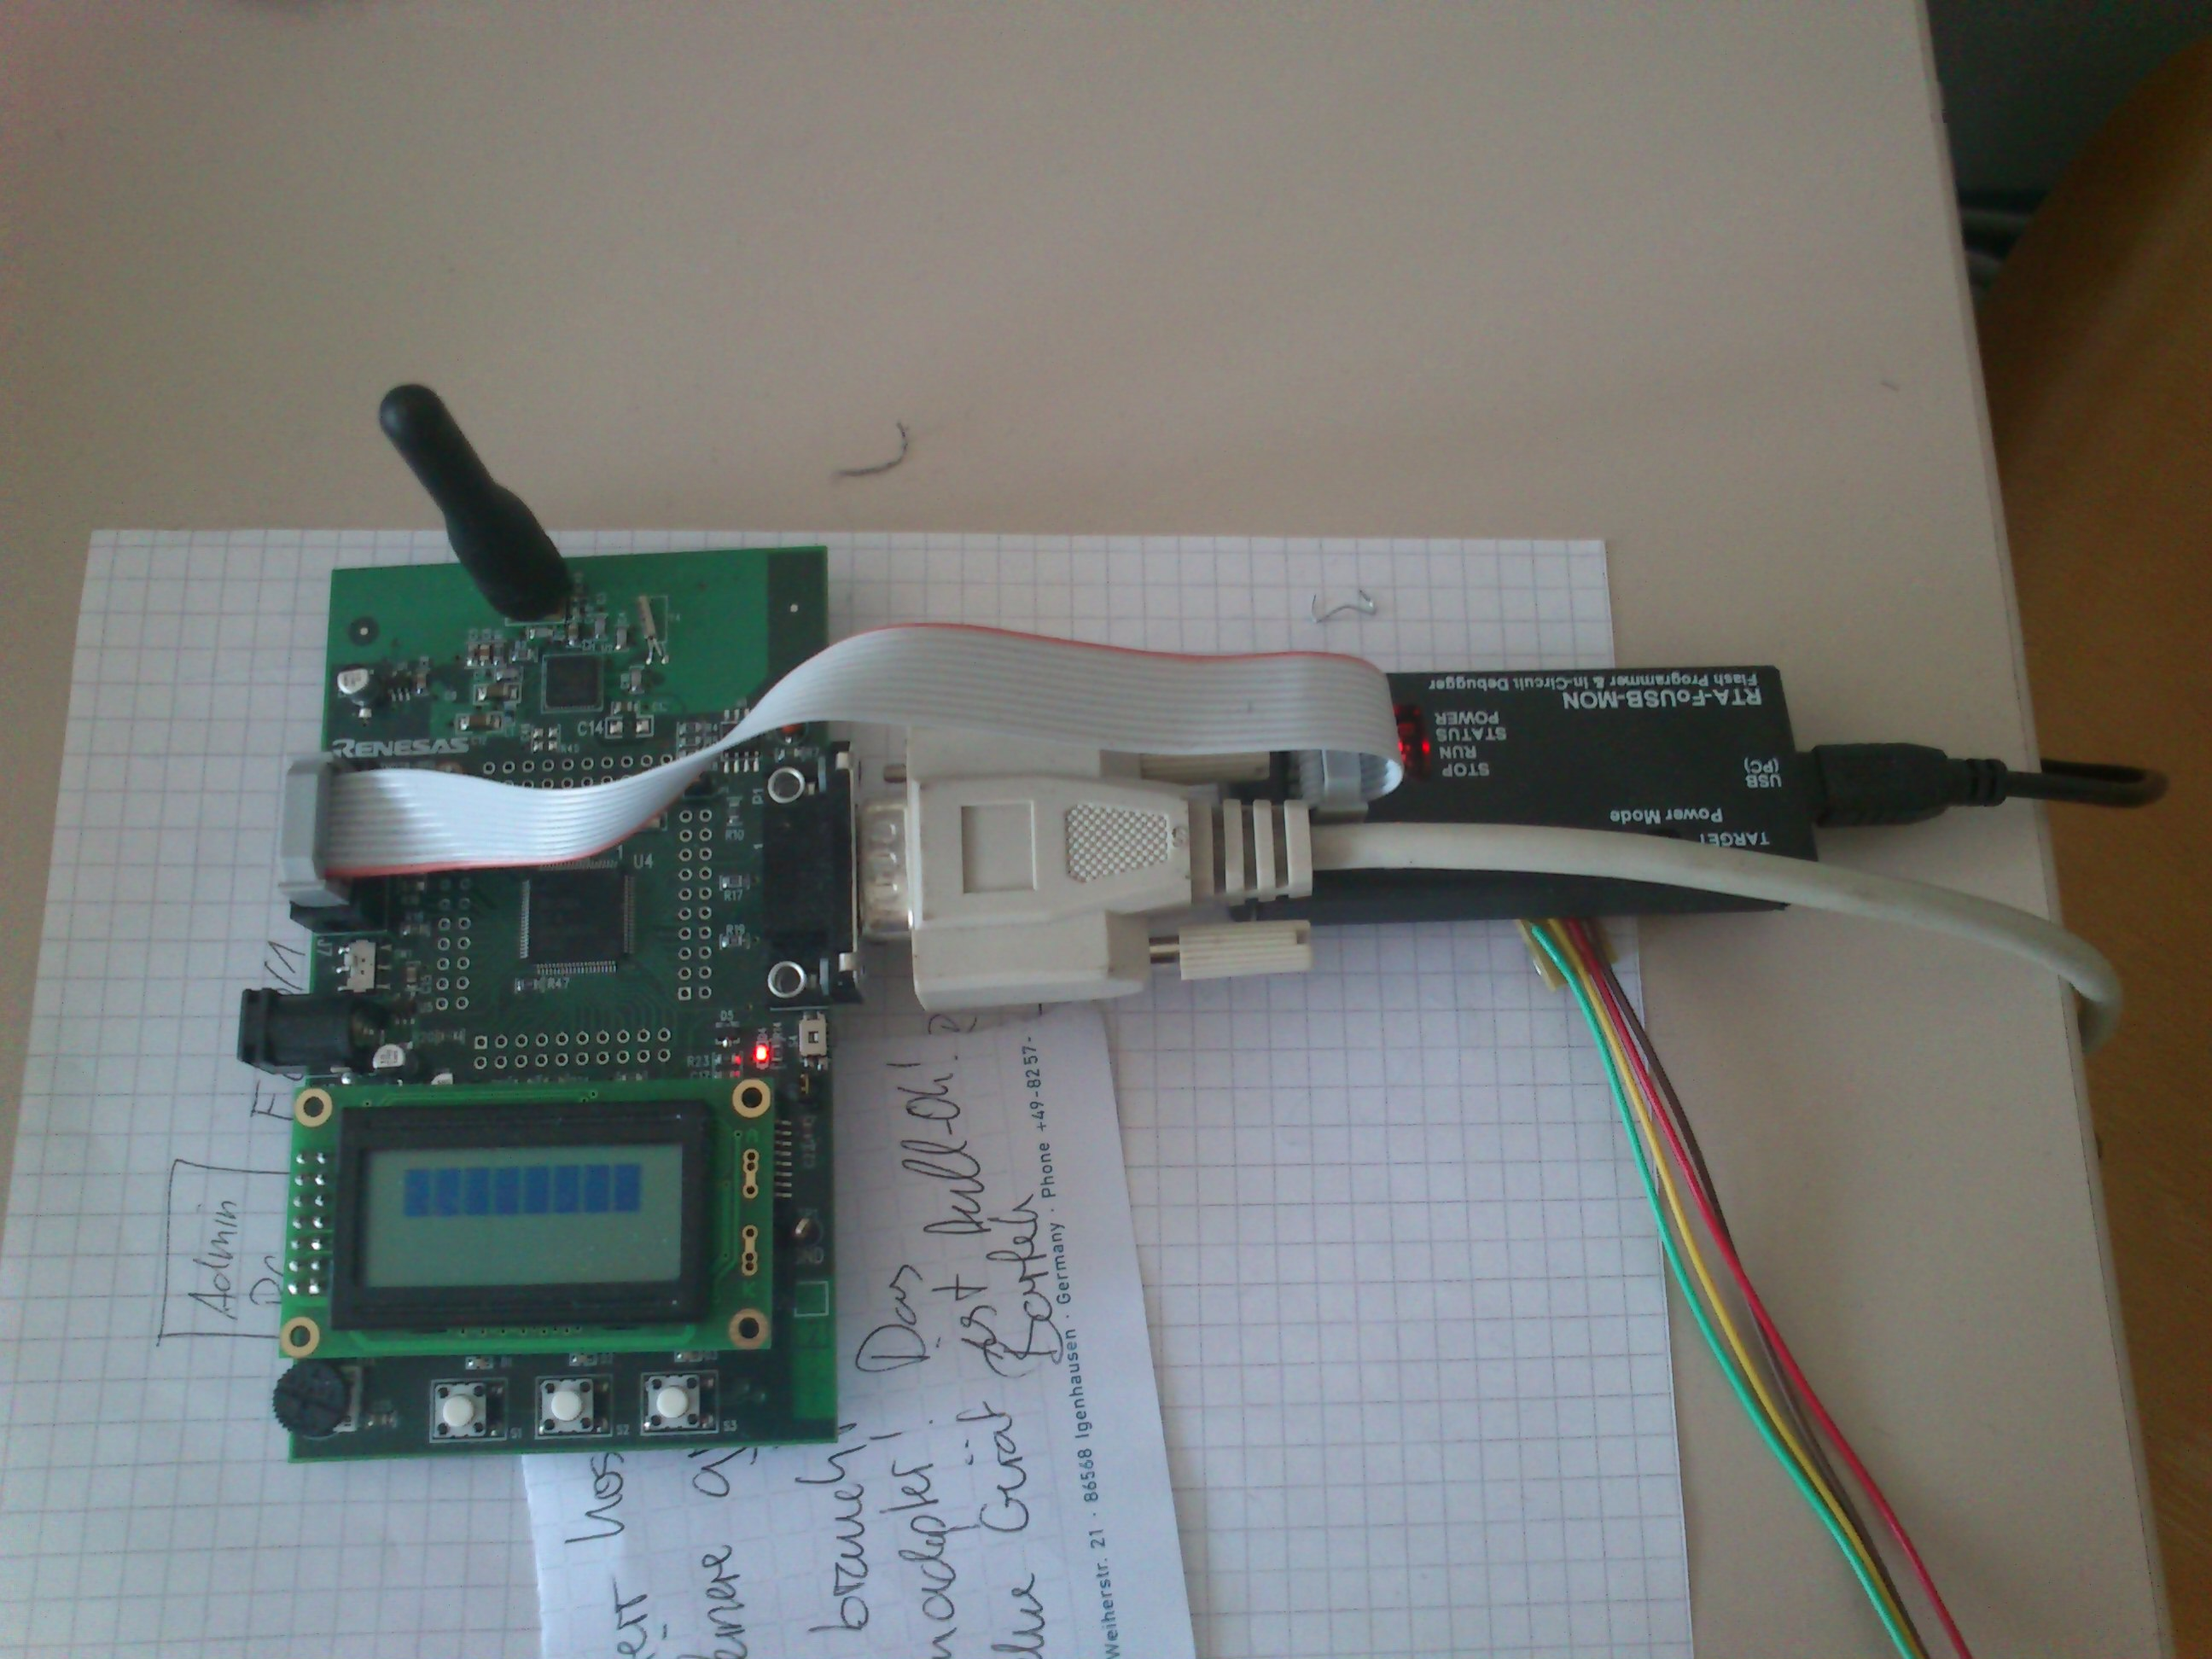
\includegraphics[width=0.8\textwidth]{pic/controller.jpg}%
   \caption{Renesas Node with Custom Programming and Serial Connector}
   \label{nodepic}%
\end{figure}

For the setup we tried to not distract ourselves from the goal so we tested with just one client. The final version is not restricted
to any finite number by the translator but only by available hardware and lower protocol stack's requirements.

\begin{figure}[H]
   \centering
   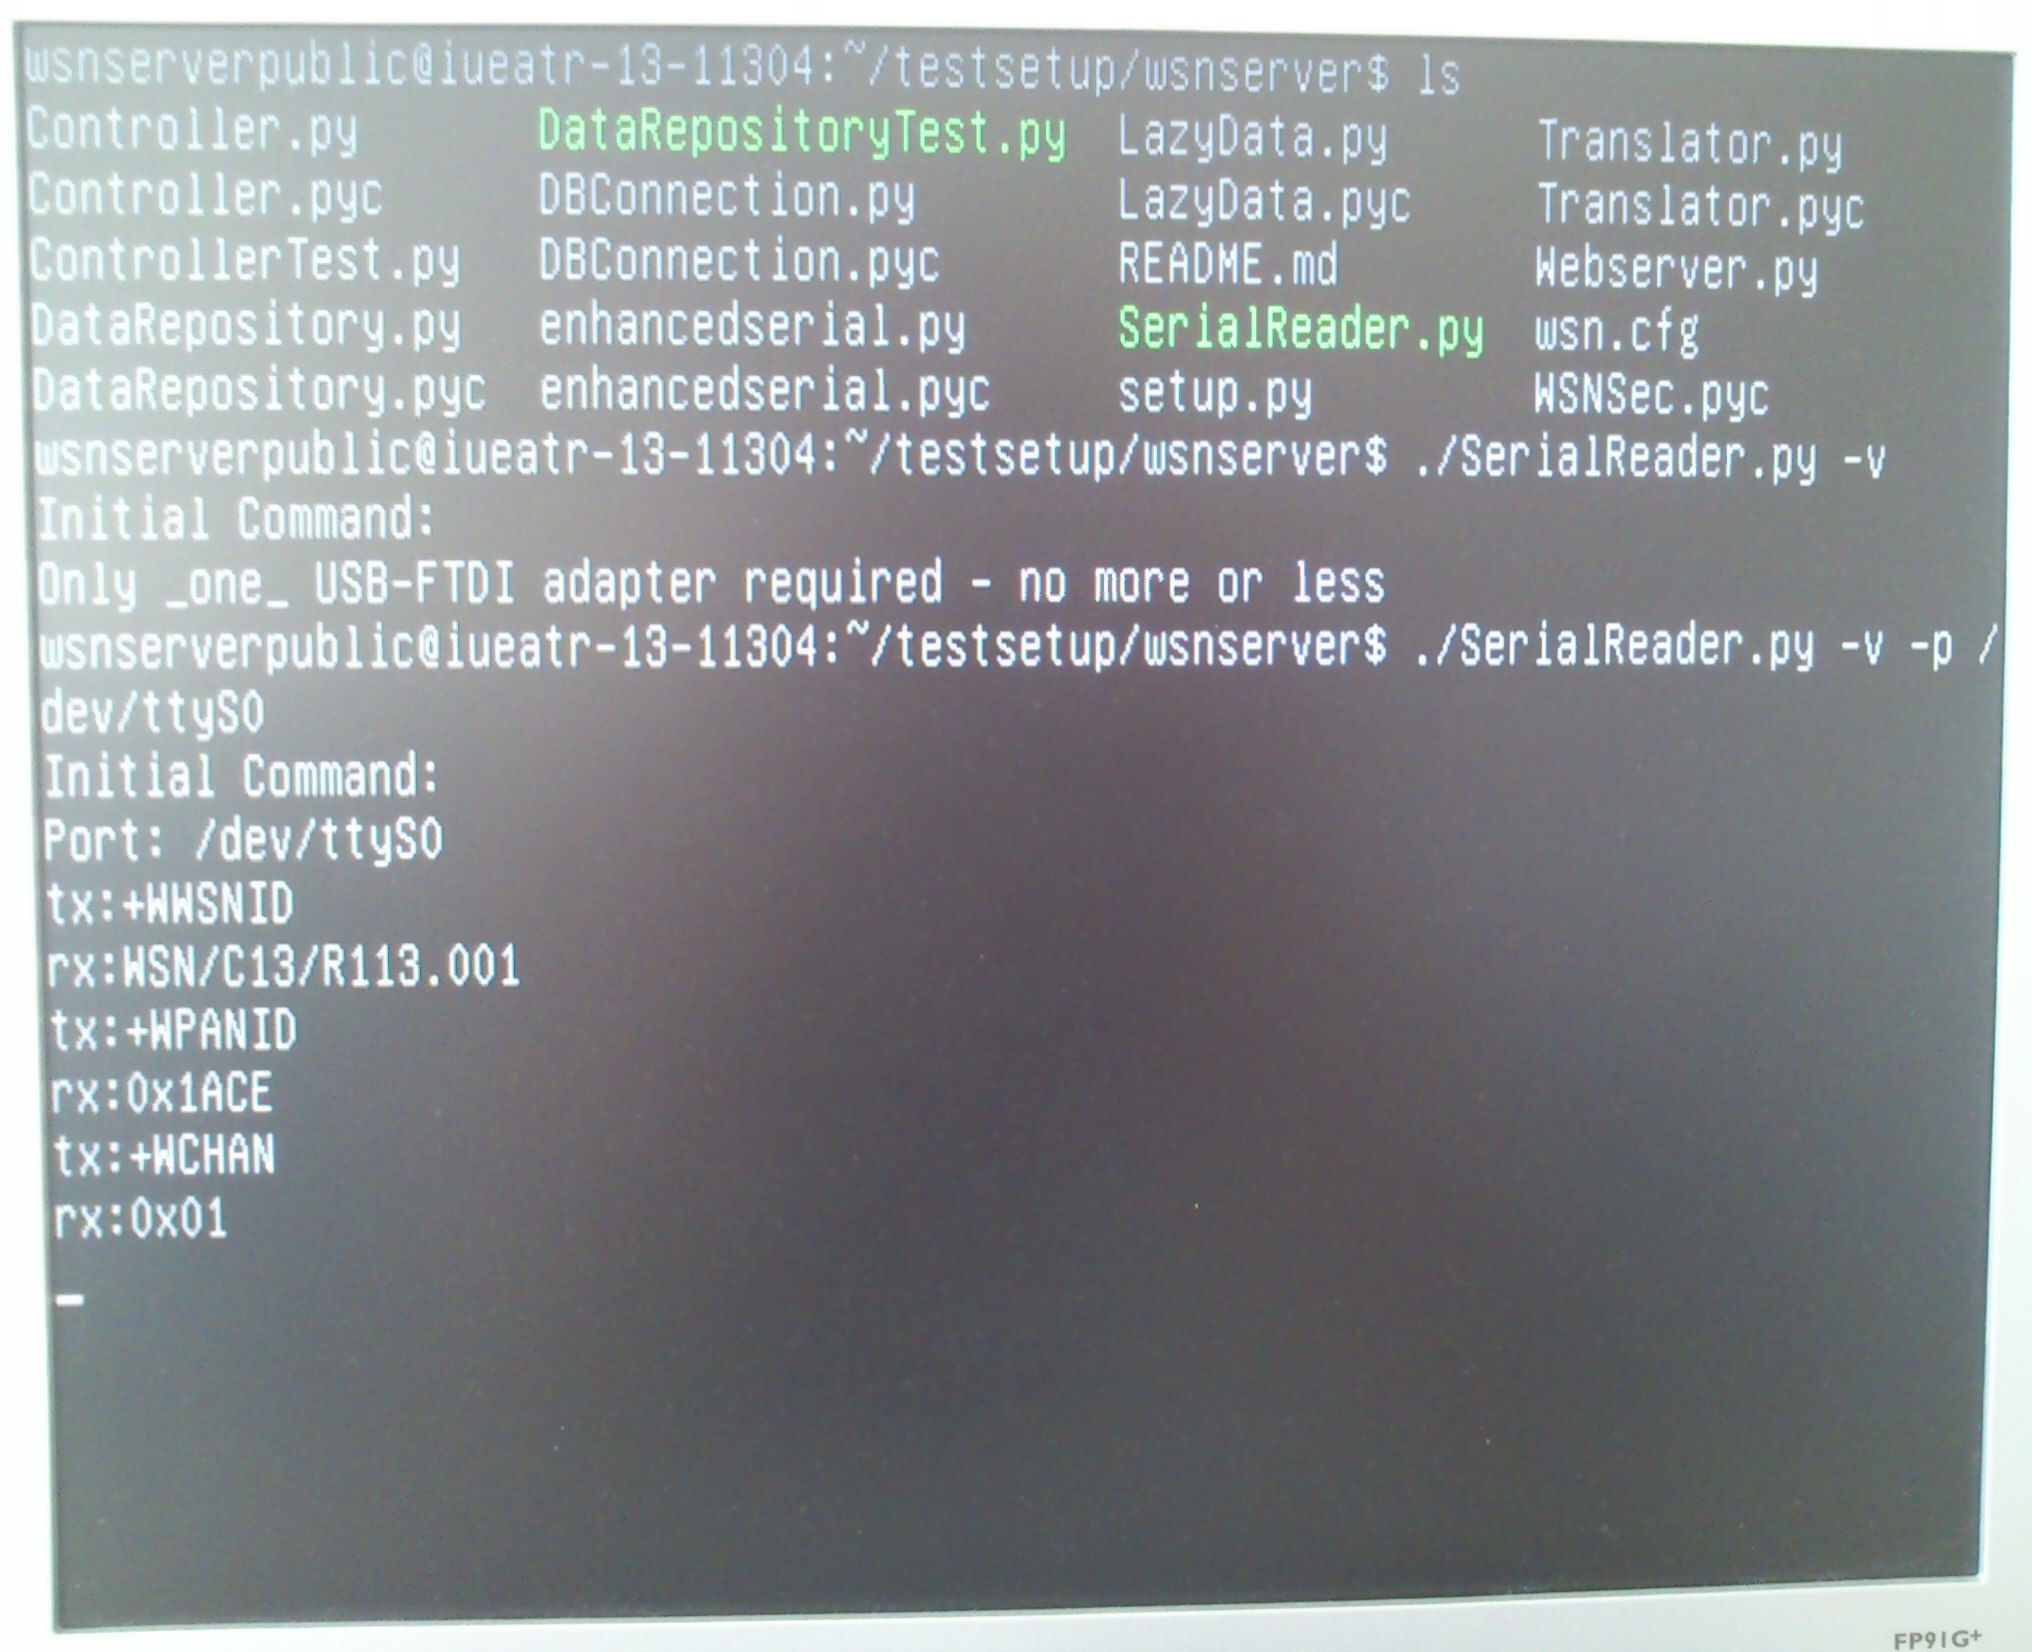
\includegraphics[width=0.8\textwidth]{pic/host_machine.jpg}%
   \caption{Console Output on Host Machine}
   \label{hostpic}%
\end{figure}

Figure~\ref{pic:hostpic} shows the state of the middleware after initialisation. On default a USB-FTDI adaptor is used to enable serial over USB.
In this test we used plain RS232 connections for accessing the controlling node. The parameters of the hardware part called \textit{SerialReader.py}
are very extensive so use the code or see a console output by using the standard \textit{--help} parameter upon start.

The next step is to identify all available nodes. Firstly, the controller gets the command \textit{+WWSNID} to report example identification numbers.
Our example shows our room number in our college where the node was resting on the table as shown in picture~\ref{pic:nodepic}. It is possible 
to use whatever means of identification but it should be unique due to its importance as database key. Every node has its own 
entry and is addressable if the lower stack on the controller/router enables it.

Furthermore visible is the ZigBee identifier for \textsc{Pan Id} and \textsc{Channel Id}. Every device has its own identifier in the ZigBee specification
but it is not required on the middleware's side. Some example output is reported by the node as you can see on the screenshot.\footnote{The screenshot
    is the debug output from the host machine. This is not the default as the host could possibly run headless. Be aware that ZigBee devices may influence
other nodes which are not part of your project. We experienced this quirk and had a lot of fun to find out why.}

\newpage
\section{The development method}

For development there have been used different approaches. Most of this project has been developed by the use of agile methods, 
what means that a feature was implemented and then tested. If it worked properly, it has been committed to a central repository. 
Critical parts like the \textit{Controller} and the \textit{DataRepository} classes have been developed by using the test-driven-development, 
where first tests have been written and afterwards the corresponding methods. This last development technique had their advantages and made 
the expansion of the \textit{DataRepository} class with a second database layer - MySQL - much easier and faster: each test case 
created for the first database layer - SQLite - had also to work with the newly implemented layer for MySQL.

The approach for the hardware backend was similar but more experimental due to the serial nature of communication between node and host machine. Only
few tests were used as there were different approaches in the life-cycle of this project: a thread-based approach was not found optimal because 
of error in the \textit{pySerial} module and hardware design flaws for threading. A buffer was inserted instead which will cache a limited amount of commands which
will be sent on the next cycle. The cycles were parted between reading and writing.

\section{Desgin concept}
[HIER KOMMT NOCH EIN UML DIAGRAMM REIN, WIE WIR UNS DAS AM ANFANG VORGESTELLT HABEN  + BEHAVIORAL DIAGRAMS (Sequensdiagram + USE CASE)- KAMILLES AUFGABE]

\section{DataBase}

[HIER KOMMT DAS DESIGN DER DATENBANK REIN -> KAMILLE]

\section{Class diagrams}
\subsection{Setup.py}
[HIER MUSS NOCH DIE SETUP.PY REIN, OBWOHL SIE NICHT SO RICHTIG ZU DEN KLASSEN PASST, DA ES SICH HIER UM EIN PROZEDURALES SKRIPT HANDELT- KAMILLES AUFGABE]

\subsection{The Controller class}
\begin{figure}[H]
   \centering
   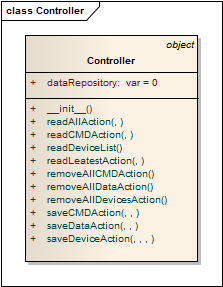
\includegraphics[width=0.5\textwidth]{pic/Controller.png}%
   \caption{The Controller class}
   \label{Controllerpic}%
\end{figure}

The \textit{Controller} class is the central part of this project. It corresponds to the controller part of the Model-View-Controller design pattern.

Like in any other MVC applications the controller receives and handles input and requests of the user and also of any other external modules. 
It validates the input and decides what to do with the data passed to the controller, 
for example if the controller should save it to the model or retrieve some data from the repository and return it as response.

Applied to this project the \textit{Controller} class receives requests from the web server to retrieve stored data for a 
WSN and also to save commands for a WSN in the database, which is used as a queue. The second actor of this class is the 
\textit{SerialReader} class, which also accesses the controller to save its identification credentials, 
to pass its read sensor data to the controller for saving and to retrieve new commands from the queue.

The last possible user is the setup script, which accesses the controller for maintenance tasks, like removing all data from the data repository.



\newpage
\subsection{The ControllerTest class}
\begin{figure}[H]
   \centering
   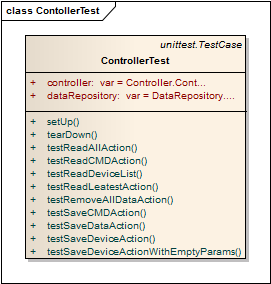
\includegraphics[width=0.5\textwidth]{pic/ControllerTest.png}%
   \caption{ControllerTest class, unittest for the Controller class}
   \label{ControllerTestpic}%
\end{figure}

This unittest was written to test the \textit{Controller} class and their functionality. 

The \textit{setUp()} method creates fixtures, which will be stored in the database, before each test case will be run. This ensures that all "retrieving"-methods have something to read and all "remove"-methods have something to delete. At the end of each test case the expected and the actual values will be compared. 

After each testrun the database will be cleared by the \textit{tearDown()} method. 

\newpage
\subsection{DataRepository class}
\begin{figure}[H]
   \centering
   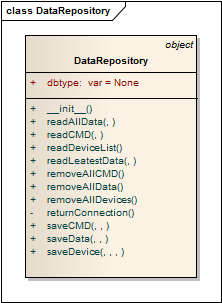
\includegraphics[width=0.5\textwidth]{pic/DataRepository.png}%
   \caption{DataRepository class, which handles the model}
   \label{DataRepositorypic}%
\end{figure}

The \textit{DataRepository} class is the main model class of this project. 
Their goal is to store and retrieve information and data from the database. 
Nearly all methods contain SQL instructions, 
which will be executed by the use of an \textit{DBConnection} object, which again contains an actual database connection.

In the first implementation the methods have been developed to run with SQLite so no other database system was needed. After running a few stresstests - by storing very much data in a very short time in the database - the database crashed. Therefore a second layer - MySQL - was developed to ensure proper function under high database usage.

\newpage
\subsection{DataRepositoryTest class}
\begin{figure}[H]
   \centering
   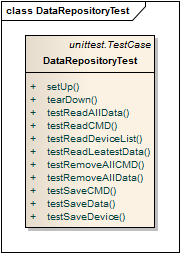
\includegraphics[width=0.5\textwidth]{pic/DataRepositoryTest.png}%
   \caption{DataRepositoryTest class, unit test for the DataRepository class}
   \label{DataRepositoryTestpic}%
\end{figure}

Equivalent to the \textit{Controller} class the \textit{DataRepository} class also possesses a test class.

The testing of the \textit{DataRepository} class was very crucial, because it was very important to ensure the proper function of the methods implemented in the \textit{DataRepository}. A small error could later cause a discrepancy when analysing the data retrieved from the database. 
The tests have been developed to be executed for the \textit{DataRepository} in its first version with SQLite, but the same tests also accelerated the development of the MySQL-layer, because every test, which has been developed to run with SQLite, had also to work identically with the MySQL-implementation.

\newpage
\subsection{DBConnection class}
\begin{figure}[H]
   \centering
   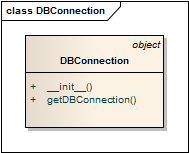
\includegraphics[width=0.5\textwidth]{pic/DBConnection.png}%
   \caption{DBConnection class, a database layer}
   \label{DBConnectionpic}%
\end{figure}

The sole purpose of the \textit{DBConnection} class is to return an open database connection to the caller. This is achieved by loading the configuration file and read out the settings, so the \textit{DBConnection} class can decide which kind of database connection it will return the the calling method as response.

\newpage
\subsection{EnhancedSerial class}
\begin{figure}[H]
   \centering
   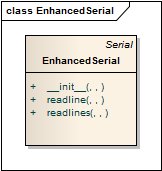
\includegraphics[width=0.5\textwidth]{pic/EnhancedSerial.png}%
   \caption{EnhancedSerial reader class}
   \label{EnhancedSerialpic}%
\end{figure}

\textit{EnhancedSerial} is a part of \url{http://pyserial.sf.net}{pyserial}  written by \href{mailto:cliechti@gmx.net}{C. Liechti} in 2002.
It is a huge improvement in comparison to the default serial line communication class. For details please look into the code.


\newpage
\subsection{LazyData class}
\begin{figure}[H]
   \centering
   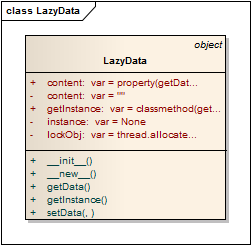
\includegraphics[width=0.5\textwidth]{pic/LazyData.png}%
   \caption{LazyData class}
   \label{LazyDatapic}%
\end{figure}

\textit{LazyData} is a singleton based on the work of Alan Felice. Mainly it serves as a data buffer for the serial output from the host to the node. 
As mentioned by~\cite{GammaHelmJohnsonVlissides199711} the singleton only allows one instance which is accessible throughout every object. It was
heavily modified by us to enable the usage for the serial reader module.

\newpage
\subsection{Translator class}
\begin{figure}[H]
   \centering
   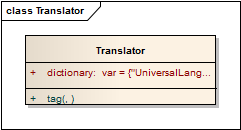
\includegraphics[width=0.5\textwidth]{pic/Translator.png}%
   \caption{Translator class}
   \label{Translatorpic}%
\end{figure}

The translation abstract class is the heart of the middleware. It enables the transition between the various language by providing a basis for further 
abstraction.

\subsubsection{MedusaTranslator class}
\begin{figure}[H]
   \centering
   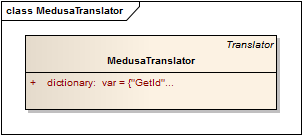
\includegraphics[width=0.5\textwidth]{pic/MedusaTranslator.png}%
   \caption{MedusaTranslator class}
   \label{MedusaTranslatorpic}%
\end{figure}

The Medusa is a node system with a lot of sonar-like \textit{heads} which are mainly used in localisation.\cite{Dispert}
This is just a symbolic help to insert also this very special node in the translation system.

\begin{figure}[H]
   \centering
   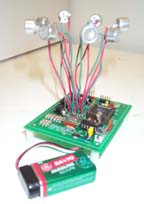
\includegraphics{pic/medusa.jpg}%
   \caption{A first generation Medusa. Image source: \url{nesl.ee.ucla.edu}}
   \label{Medusapic}%
\end{figure}


\subsubsection{RenesasTranslator class}
\begin{figure}[H]
   \centering
   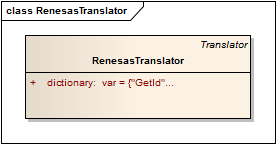
\includegraphics[width=0.5\textwidth]{pic/RenesasTranslator.png}%
   \caption{RenesasTranslator class, dictionary class for Renesas}
   \label{RenesasTranslatorpic}%
\end{figure}

As the Renesas ZMD28-BRD is used as our main development board we included a full class for temperature sensing. It is a very 
basic hardware programming on the node to not complicate the whole project. It was provided by the laboratory assistant Stephan Ko\ss.

The class itself is mainly a dictionary which is used for the translation process.

\newpage
\subsection{SerialReader class}
\begin{figure}[H]
   \centering
   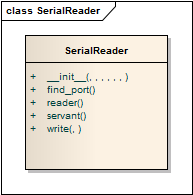
\includegraphics[width=0.5\textwidth]{pic/SerialReader.png}%
   \caption{SerialReader class, main class for reading data from serial port}
   \label{SerialReaderpic}%
\end{figure}

\textit{SerialReader} is used for the hardware part. It is highly configurable through parameters and even more through code. As the
serial RS232 connector utilizes a big amount of different configuration parameters a possible adaptor will surely have to look inside the
programming. It is the main component which must be started.\footnote{Also the database is important if you don't want to rely on sqlite.}

\newpage
\subsection{Webserver class}
\begin{figure}[H]
   \centering
   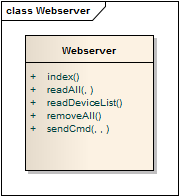
\includegraphics[width=0.5\textwidth]{pic/Webserver.png}%
   \caption{Webserver class, containing the web server}
   \label{web serverpic}%
\end{figure}

The \textit{Webserver} class can be seen as the \textit{View} part of the MVC pattern, as it allows and restricts the access and the requests of a user to this specified methods.

The class uses the CherryPy web server framework.\footnote{The CherryPy web server is a open source project hosted on \url{http://www.cherrypy.org/}} A standalone web server written completely in Python. The advantage of this fact is that the dependency of project is reduced to Python instead of the use of a big and resource hungry web server like Apache2. Also the easy and fast development of methods/pages which comes with the framework.

For demonstration of the simplicity of CherryPy an extract of the \textit{Webserver} class is presented. As it can be seen, it is already enough to define a method to receive a functional site. 
\begin{lstlisting}[language=Python]
import Controller
import cherrypy
from cherrypy import expose

class web server:
    @expose
    def index(self):
        return "WSN-Server is up and running"
       
\end{lstlisting}

To see if this method works, the user has to call \url{http://localhost:8080/index} and will receive the status of the web server.

\newpage
\section{Custom Installation}
\label{sec:install}

Custom installation is only required when not using the provided disc image.

\begin{enumerate}
    \item Install a Linux of your chosen flavour. Preferably use Debian.
    \item Install git\footnote{\textit{apt-get install git}}
    \item Download and install cherrypy\footnote{\url{http://www.cherrypy.org/wiki/CherryPyDownload} or on Debian \textit{apt-get install python-cherrypy}}
    \item Run \textit{python setup.py --sqlite} to create and configure the SQLite database. For further information or help run \textit{python setup.py -h}, which explains the usage of the commandline script.\footnote{This step is only required if you do not use the MySQL backend}
    \item \textit{Optionally:} Install a MySQL server and proper SQL bindings for increased functionality\footnote{\textit{apt-get install mysql-server mysql-client libmysqlclient15-dev python-mysqldb}}
\end{enumerate}

The last step is to use a proper user-account\footnote{root not recommended but put the user in the appropriate group for accessing serial connection} and
get the most recent development version with git.\footnote{\textit{git clone git@github.com:Phialo/wsnserver.git}}

Finally, you change directory to the project and run \textit{python SerialReader.py -h} to see available options.

If there is a need to make all the gathered data and informations available for further use, the \textit{web server} can be started by running \textit{python Webserver.py}. This will automatically start the 
\textit{web server} and make all implemented methods immediately ready for use. To see which commands respectively methods are available, the user should take a look at the description of the \textit{Webserver} class.
